\section{Experiments on SPO-chain}
\label{sec:experiments_on_spo_chain}

\textbf{Experimental Setups.}
We evaluate SPO-chain with the RhoMath 1.1B model \cite{lin2025rho1tokensneed} on the GSM8K dataset \cite{cobbe2021trainingverifierssolvemath} using Pass@1 (accuracy) as our primary evaluation metric. Following \cite{kazemnejad2024vineppounlockingrlpotential}, we first finetune the base model on the GSM8K training set, and then use the obtained SFT model for subsequent RL training. We compare against baseline methods including RestEM, DPO, PPO, GRPO, RLOO, and VinePPO. The experimental hyperparameters largely follow \cite{kazemnejad2024vineppounlockingrlpotential}, with detailed settings provided in Appendix \ref{appendix:hyperparameter}. For SPO-chain, we set the number of MC samples to $N=9$ and partitioned the model output at \textbf{intervals of every 5 cutpoints}, which is referred to as \textbf{SPO-chain (int5)}. We also evaluate our SPO-tree method in the short CoT scenario. We adopt a 6-6-6 tree structure, meaning the tree consists of three layers and each internal node expands into six child nodes, which is referred to as \textbf{SPO-tree (6-6-6)}. For the first two layers, we segment the model output every 30 tokens, while for the final layer, we let the model complete the entire reasoning trajectory.

\begin{figure}[!t]
  \centering
  \begin{minipage}[t]{0.32\textwidth}
    \centering
    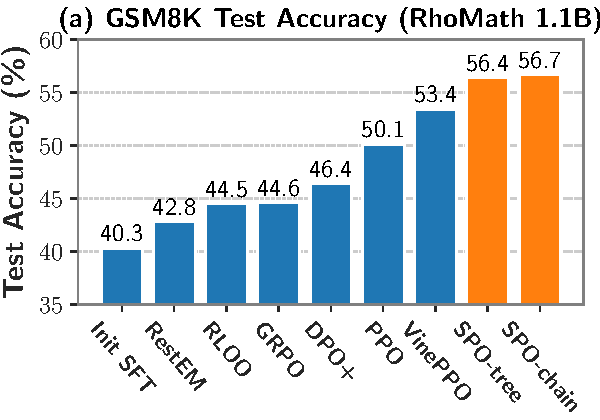
\includegraphics[width=\textwidth]{eval-figures/GSM8K-acc-only-bar.pdf}
  \end{minipage}\hfill
  \begin{minipage}[t]{0.32\textwidth}
    \centering 
    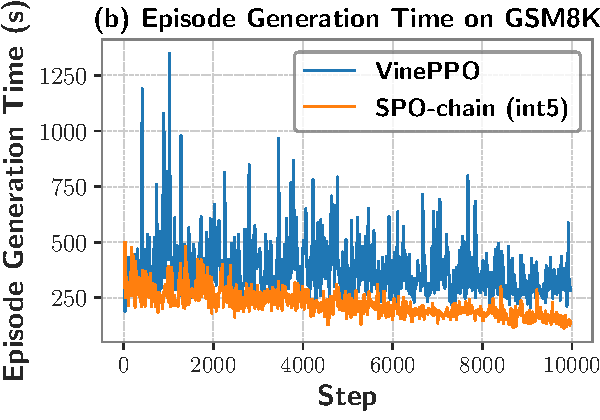
\includegraphics[width=\textwidth]{eval-figures/GSM8K-vineppo-time.pdf}
  \end{minipage}\hfill
  \begin{minipage}[t]{0.32\textwidth}
        \centering
        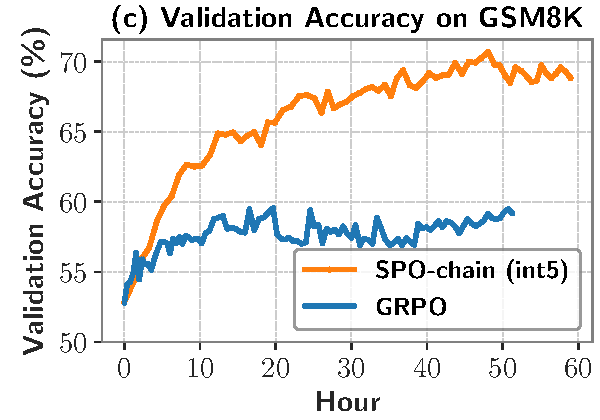
\includegraphics[width=\textwidth]{eval-figures/GRPO-SPO-chain-acc-line.pdf}
    \end{minipage}%
    \caption{\textbf{(a)} Test accuracy comparison of different methods on GSM8K. Baseline results are from \cite{kazemnejad2024vineppounlockingrlpotential}. \textbf{(b)} Episode generation time comparison between SPO-chain (int5) and VinePPO during training. \textbf{(c)} Validation accuracy of SPO-chain (int5) and GRPO during training.}
    \label{fig:GSM8K-accuracy-results}
\end{figure}

\begin{figure}[!t]
    \centering
    \begin{minipage}[t]{0.32\textwidth}
        \centering
        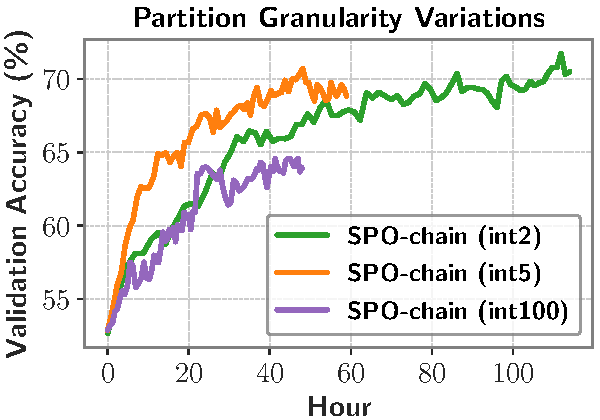
\includegraphics[width=\textwidth]{eval-figures/interval_wall_time.pdf}
        \label{fig:segment_interval}
    \end{minipage}
    \hfill
    \begin{minipage}[t]{0.32\textwidth}
        \centering
        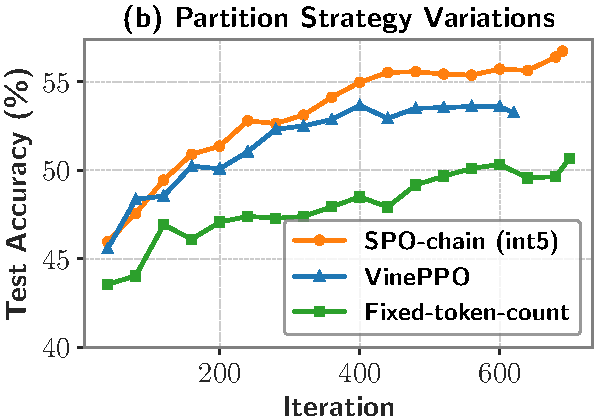
\includegraphics[width=\textwidth]{eval-figures/Segment-methods-var.pdf}
        \label{fig:segment_method}
    \end{minipage}
    \hfill 
    \begin{minipage}[t]{0.32\textwidth}
        \centering
        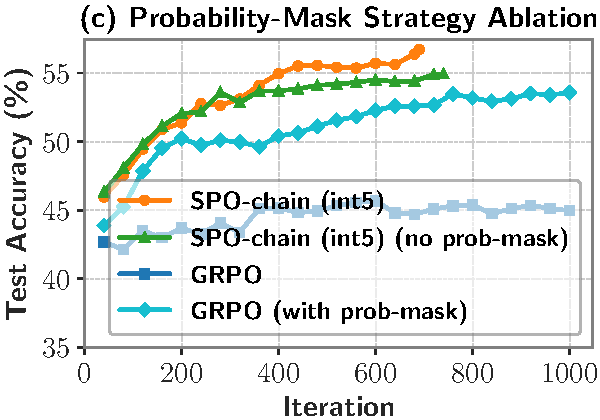
\includegraphics[width=\textwidth]{eval-figures/Segment-prob-mask.pdf}
        \label{fig:prob_mask}
    \end{minipage}%
    \vspace{-1em}
    \caption{\textbf{(a)} Variations of segment partition granularity (different cutpoint intervals). \textbf{(b)} Variations of segment partition strategies. \textbf{(c)} Ablation on probability-mask policy optimization strategy.}
    \vspace{-0.5cm}
\end{figure}

\textbf{Comparison with Baseline Methods.}
As shown in Figure \hyperref[fig:GSM8K-accuracy-results]{3(a)}, our method, SPO-chain (int5), achieves the highest accuracy on the GSM8K test set, outperforming PPO and GRPO by 6-12 percentage points. Furthermore, compared to VinePPO, our method not only delivers higher accuracy but also requires less time for episode generation, as demonstrated in Figure \hyperref[fig:GSM8K-accuracy-results]{3(b)}. This is due to our SPO-chain (int5) method uses fewer advantage estimation points per trajectory compared to VinePPO. Additionally, our SPO-tree (6-6-6) method achieves the second-highest accuracy on the GSM8K test set, validating its effectiveness and making it an efficient alternative. We also compared our method with GRPO in terms of validation performance under the same wall-clock time\footnote{Evaluation time is also included in the reported wall-clock time. The model is evaluated every 10 iterations.} (Figure \hyperref[fig:GSM8K-accuracy-results]{3(c)}). The results show that our algorithm significantly outperforms GRPO and ultimately converges to a much better solution. We further conduct experiments with additional models, including DeepSeekMath 7B \cite{shao2024deepseekmathpushinglimitsmathematical}, Qwen base and instruct models \cite{qwen3technicalreport}, as well as on the non-mathematical Knights-and-Knaves dataset \cite{xie2024memorization}. The detailed results of these experiments are presented in Appendix~\ref{appendix:addition_experiments_results}.

\textbf{Impact of Segmentation Granularity.} 
To investigate how the segment granularity affects model performance, we conducted experiments using various segment intervals, as shown in \hyperref[fig:segment_interval]{4(a)}. When comparing validation accuracy under the same wall-clock time, interval 5 achieves the highest performance, followed by interval 2, while interval 100 performs the worst. In terms of final accuracy, interval 2 slightly surpasses interval 5, whereas interval 100 lags significantly behind both. These results indicate that a moderate interval (e.g., 5) provides a more favorable trade-off, yielding better accuracy given the same training time, while excessively fine-grained intervals (e.g., 2) bring only marginal improvements and overly coarse intervals severely harm the accuracy. This supports the design of our segment-level advantage method, which strikes an effective balance between efficiency and accuracy, achieving substantially better performance than trajectory-level advantage without the high computational cost of token-level estimation.

\textbf{Comparison of Different Segment Partition Strategies.} 
We compare different trajectory partition methods, including the naive fixed token count partition, the heuristic rules (e.g. line breaks) for partitioning as in VinePPO, and the cutpoint-based segment partition in SPO-chain. The results are presented in Figure \hyperref[fig:segment_interval]{4(b)}. For the naive fixed token count partitioning method, we explicitly set each trajectory's segment count at 3, making it higher than the total sampling budget of the SPO-chain (int5). Remarkably, despite having the smallest sampling budget, SPO-chain (int5) achieves the best test accuracy, validating the effectiveness of our cutpoint-based segment partition strategy.

\textbf{Ablation Study on Probability-Mask Optimization Strategy.} 
We conduct an ablation study on our proposed probability-mask optimization technique. As shown in Figure \hyperref[fig:segment_interval]{4(c)}, removing the probability-mask technique leads to a decreased accuracy for SPO-chain (int5), from 56.7\% to 55.0\%. Surprisingly, applying the probability-mask technique to GRPO results in a significant improvement, boosting its accuracy from 45.7\%\footnote{Our GRPO implementation achieves a slightly higher test accuracy (45.7\%) compared to the 44.6\% reported in \cite{kazemnejad2024vineppounlockingrlpotential}.} to 53.6\%. We hypothesize that employing the probability-mask technique enables more precise credit assignment to tokens that are most likely to influence the model’s reasoning trajectory. Meanwhile, the losses associated with tokens whose probabilities are close to 1 are masked out and thus excluded from the overall loss function, which potentially helps reduce overfitting.